\begin{task}
\TT{Wyznacz współczynniki trygonometrzycznego szeregu Fouriera dla okresowego sygnału $f(t)$ przedstawionego na rysunku.}{Calculate coefficients of the periodic signal $f(t)$ shown below for the expansion into a trigonometric Fourier series.} 

\begin{figure}[H]
\centering
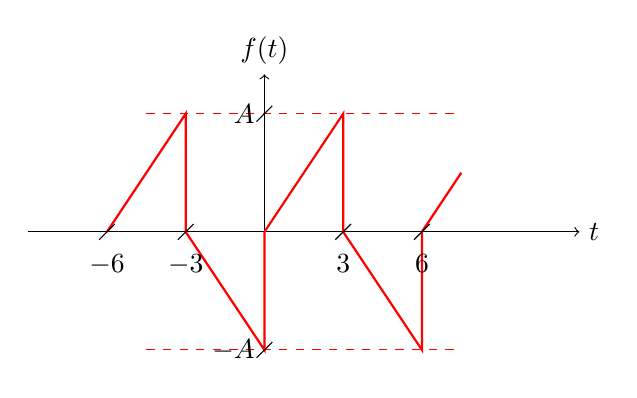
\begin{tikzpicture}
  %\draw (0,0) circle (1in);
  \draw[->] (-3.0,+0.0) -- (4.0,+0.0) node[right] {$t$};
  \draw[->] (+0.0,-1.5) -- (+0.0,+2.0) node[above] {$f(t)$};
  \draw[-,red, thick] (-2.0,0.0) -- (-1.0,1.5)--(-1.0,0.0) -- (0.0,-1.5) -- (0.0,+0.0) -- (+1.0,+1.5) -- (+1.0,+0.0) -- (+2.0,-1.5) -- (+2.0,+0.0) -- (2.5,0.75);
  \draw[-,red, dashed] (-1.5,1.5) -- (2.5,1.5);
  \draw[-,red, dashed] (-1.5,-1.5) -- (2.5,-1.5);

  \draw[-] (-2.0-0.1,-0.1)--(-2.0+0.1,0.1) node[midway, below, outer sep=5pt] {$-6$};
  \draw[-] (-1.0-0.1,-0.1)--(-1.0+0.1,0.1) node[midway, below, outer sep=5pt] {$-3$};
  \draw[-] (+1.0-0.1,-0.1)--(+1.0+0.1,0.1) node[midway, below, outer sep=5pt] {$3$};
  \draw[-] (+2.0-0.1,-0.1)--(+2.0+0.1,0.1) node[midway, below, outer sep=5pt] {$6$};
  \draw[-] (-0.1,+1.5-0.1)--(+0.1,+1.5+0.1) node[midway, left] {$A$};
  \draw[-] (-0.1,-1.5-0.1)--(+0.1,-1.5+0.1) node[midway, left] {$-A$};

\end{tikzpicture}
\end{figure}

\TT{W pierwszej kolejności należy ustalić wzór funkcji przedstawionej na rysunku. Jest to funkcja przedziałowa. W pierwszym okresie możemy ją opisać za pomocą dwóch prostych. Ogólne równanie prostej to:}{First of all, the definition of $f(t)$ signal has to be derived. This is periodic piecewise function, piecewise linear function to be precise.
The simplest form of a linear function is:}

\begin{equation}
f(t) = a \cdot t + b
\end{equation}

\TT{W pierwszym okresie, w pierwszej części, wykres funkcji jest prostą przechodzącą przez dwa punkty: $(0,0)$ oraz $(3,A)$. Możemy więc napisać układ równań, rozwiązać go i znaleźć nieznane parametry $a$ i $b$. }{In the first interval of the first period (e.g. $t \in (0; 3)$), linear function crosses two points: $(0,0)$ and $(3,A)$. So, in order to derive $a$ and $b$, the following system of the equations has to be solved.}  

\begin{align*}
&\left\{\begin{matrix*}[l]
0 = a\cdot 0 +b\\ 
A = a\cdot 3 +b
\end{matrix*}\right. \\
&\left\{\begin{matrix*}[l]
0 = b\\ 
A = a \cdot 3 +b
\end{matrix*}\right. \\
&\left\{\begin{matrix*}[l]
0 = b\\ 
A = a \cdot 3 +0
\end{matrix*}\right. \\
&\left\{\begin{matrix*}[l]
0 = b\\ 
\frac{A}{3} = a
\end{matrix*}\right.
\end{align*}

\TT{Podsumowując, pierwszy odcinek funkcji przedstawionej na rysunku, w pierwszym okresie można opisać wzorem:}{As a result we get:}
\begin{align*}
f(t) = \frac{A}{3}\cdot t
\end{align*}

\TT{Drugi odcinek funkcji jest prostą przechodzącą przez następujące dwa punkty: $(3,0)$ oraz $(6,-A)$. Możemy więc napisać układ równań, rozwiązać go i znaleźć nieznane parametry $a$ i $b$.}{In the second interval of the first period (e.g. $t \in (3; 6)$), linear function crosses other two points:: $(3,0)$ and $(6,-A)$. So, in order to derive $a$ and $b$, the following system of the equations has to be solved.}

\begin{align*}
&\left\{\begin{matrix*}[l]
0 = a\cdot 3 +b\\ 
-A = a\cdot 6 +b
\end{matrix*}\right. \\
&\left\{\begin{matrix*}[l]
-3 \cdot a = b\\ 
-A = 6 \cdot a -3 \cdot a
\end{matrix*}\right. \\
&\left\{\begin{matrix*}[l]
-3 \cdot a = b\\ 
-A = 3 \cdot a
\end{matrix*}\right. \\
&\left\{\begin{matrix*}[l]
-3 \cdot a = b\\  
-\frac{A}{3} = a
\end{matrix*}\right. \\
&\left\{\begin{matrix*}[l]
-3 \cdot (-\frac{A}{3}) = b\\
-\frac{A}{3} = a
\end{matrix*}\right. \\
&\left\{\begin{matrix*}[l]
A = b\\
-\frac{A}{3} = a
\end{matrix*}\right.
\end{align*}

\TT{A więc drugi odcinek funkcji przedstawionej na rysunku w pierwszym okresie, można opisać wzorem:}{As a result, second interval of the first period is described by:}

\begin{align*}
f(t) = -\frac{A}{3}\cdot t + A
\end{align*}

\TT{W związku z tym, całą funkcję w pierwszym okresie można zapisać jako funkcje przedziałową:}{As a result the piecewise linear function in the first period is given by:}

\begin{align*}
f(t) = \left\{\begin{matrix*}[l]
\frac{A}{3}\cdot t & for &t \in (0;3)\\ 
-\frac{A}{3}\cdot t + A & for & t \in (3; 6)
\end{matrix*}\right.
\end{align*}

\TT{I ogólniej, całą funkcję można wyrazić następującym wzorem:}{For the whole periodic signal $f(t)$ we get:}

\begin{align*}
f(t) = \left\{\begin{matrix*}[l]
\frac{A}{3}\cdot \left( t - k\cdot 6 \right) & for &t \in (0 + k\cdot 6; 3 + k\cdot 6)\\ 
-\frac{A}{3}\cdot \left( t - k\cdot 6 \right) + A & for & t \in (3 + k \cdot 6; 6+ k\cdot 6)
\end{matrix*}\right. \wedge k \in \TT{I}{Z}
\end{align*}

\TT{Współczynnik $a_0$ wyznaczamy ze wzoru}{The $a_0$ coefficient is defined as:}

\begin{equation}
a_0=\frac{1}{T}\int_{T}f(t) \cdot dt
\end{equation}

\TT{Podstawiamy do wzoru wzór naszej funkcji w pierwszym okresie $k=0$}{For the period $t \in \left(0;6\right)$, i.e. $k=0$, we get:}

\begin{align*}
a_0&=\frac{1}{T}\int_{T}f(t) \cdot dt\\
&=\frac{1}{6} \cdot \left[ \int_{0}^{3}\frac{A}{3}\cdot t \cdot dt
+\int_{3}^{6}\left(-\frac{A}{3}\cdot t + A\right) \cdot dt \right]=\\
&=\frac{A}{18} \cdot \int_{0}^{3} t \cdot dt
- \frac{A}{18} \cdot \int_{3}^{6} t \cdot dt + \frac{A}{6} \cdot \int_{3}^{6} dt=\\
&=\frac{A}{18} \cdot \left. \frac{t^2}{2} \right|_{0}^{3}
- \frac{A}{18} \cdot \left. \frac{t^2}{2} \right|_{3}^{6} + \frac{A}{6} \cdot \left. t \right|_{3}^{6}=\\
&=\frac{A}{36} \cdot \left( 3^2 - 0^2 \right) - \frac{A}{36} \cdot \left( 6^2 - 3^2 \right) + \frac{A}{6} \cdot \left( 6 - 3\right)=\\
&=\frac{A}{36} \cdot 9 - \frac{A}{36} \cdot 27 + \frac{A}{6} \cdot 3=\\
&=\frac{9 \cdot A}{36} - \frac{27 \cdot A}{36} + \frac{18 \cdot A}{36}=\\
&=0
\end{align*}

\TT{Wartość współczynnika $a_0$ wynosi $0$}{The $a_0$ coefficient equals $0$.}

\TT{Współczynnik $a_k$ wyznaczamy ze wzoru}{The $a_k$ coefficients are defined as:}

\begin{equation}
a_k=\frac{2}{T}\int_{T}f(t) \cdot cos\left( k \cdot \frac{2\pi}{T} \cdot t\right) \cdot dt
\end{equation}

\TT{Podstawiamy do wzoru wzór naszej funkcji w pierwszym okresie $k=0$}{For the period $t \in \left(0;6\right)$, i.e. $k=0$, we get:}

\begin{align*}
a_k&=\frac{2}{T}\int_{T}f(t) \cdot cos\left( k \cdot \frac{2\pi}{T} \cdot t\right) \cdot dt\\
&=\frac{2}{6} \cdot \left[\int_{0}^{3}\frac{A}{3}\cdot t \cdot cos\left( k \cdot \frac{2\pi}{6} \cdot t\right) \cdot dt
+\int_{3}^{6}\left(-\frac{A}{3}\cdot t + A\right) \cdot cos\left( k \cdot \frac{2\pi}{6} \cdot t\right) \cdot dt \right]=\\
&=\frac{A}{9} \cdot \int_{0}^{3} t \cdot cos\left( k \cdot \frac{\pi}{3} \cdot t\right) \cdot dt
- \frac{A}{9} \cdot \int_{3}^{6} t \cdot cos\left( k \cdot \frac{\pi}{3} \cdot t\right) \cdot dt + \frac{A}{3} \cdot \int_{3}^{6} cos\left( k \cdot \frac{\pi}{3} \cdot t\right) dt=\\
&=\begin{Bmatrix*}[l]
u&=t & dv&=cos\left( k \cdot \frac{\pi}{3} \cdot t\right) \cdot dt \\
du&=dt & v&=\frac{3}{k\cdot \pi}\cdot sin\left( k \cdot \frac{\pi}{3} \cdot t\right)
\end{Bmatrix*}=\\
&=\frac{A}{9} \cdot \left[ \left. t \cdot \frac{3}{k\cdot \pi}\cdot sin\left( k \cdot \frac{\pi}{3} \cdot t\right) \right|_{0}^{3} - \int_{0}^{3}  \frac{3}{k\cdot \pi}\cdot sin\left( k \cdot \frac{\pi}{3} \cdot t\right) \cdot dt \right]-\\
&-\frac{A}{9} \cdot \left[ \left. t \cdot \frac{3}{k\cdot \pi}\cdot sin\left( k \cdot \frac{\pi}{3} \cdot t\right) \right|_{3}^{6} - \int_{3}^{6}  \frac{3}{k\cdot 3\pi}\cdot sin\left( k \cdot \frac{\pi}{3} \cdot t\right) \cdot dt \right]+\\
&+ \frac{A}{3} \cdot \left. \frac{3}{k\cdot \pi}\cdot sin\left( k \cdot \frac{\pi}{3} \cdot t\right) \right|_{3}^{6}=\\
&=\frac{3 \cdot A}{9 \cdot k \cdot \pi} \cdot \left[ 3 \cdot sin\left( k \cdot \frac{\pi}{3} \cdot 3\right) -  0 \cdot sin\left( k \cdot \frac{\pi}{3} \cdot 0\right)
 + \left. \frac{3}{k\cdot \pi}\cdot cos\left( k \cdot \frac{\pi}{3} \cdot t\right) \right|_{0}^{3}\right]-\\
&-\frac{3 \cdot A}{9 \cdot k \cdot \pi} \cdot \left[ 6 \cdot sin\left( k \cdot \frac{\pi}{3} \cdot 6\right) -  3 \cdot sin\left( k \cdot \frac{\pi}{3} \cdot 3\right)
+ \left. \frac{3}{k\cdot \pi}\cdot cos\left( k \cdot \frac{\pi}{3} \cdot t\right) \right|_{3}^{6}\right]+\\
&+ \frac{A}{k\cdot \pi} \cdot \left[sin\left( k \cdot \frac{\pi}{3} \cdot 6\right) - sin\left( k \cdot \frac{\pi}{3} \cdot 3\right)\right]=\\
&=\frac{A}{3 \cdot k \cdot \pi} \cdot \left[ 3 \cdot sin\left( k \cdot \pi\right) -  0 
+ \frac{3}{k\cdot \pi}\cdot cos\left( k \cdot \frac{\pi}{3} \cdot 3\right) -  \frac{3}{k\cdot \pi}\cdot cos\left( k \cdot \frac{\pi}{3} \cdot 0\right)\right]-\\
&-\frac{A}{3 \cdot k \cdot \pi} \cdot \left[ 6 \cdot sin\left( k \cdot 2 \pi \right) -  3 \cdot sin\left( k \pi \right) + \frac{3}{k\cdot \pi}\cdot cos\left( k \cdot \frac{\pi}{3} \cdot 6\right) - \frac{3}{k\cdot \pi}\cdot cos\left( k \cdot \frac{\pi}{3} \cdot 3\right)\right]+\\
&+ \frac{A}{k\cdot \pi} \cdot \left[sin\left( k \cdot 2\pi\right) - sin\left( k \cdot \pi \right)\right]=\\
&=\frac{A}{3 \cdot k \cdot \pi} \cdot \left[ 3 \cdot 0 + \frac{3}{k\cdot \pi}\cdot cos\left( k \cdot \pi\right) -  \frac{3}{k\cdot \pi}\cdot cos\left(0\right)\right]-\\
&-\frac{A}{3 \cdot k \cdot \pi} \cdot \left[ 6 \cdot 0 -  3 \cdot 0 + \frac{3}{k\cdot \pi}\cdot cos\left( k \cdot 2 \pi \right) - \frac{3}{k\cdot \pi}\cdot cos\left( k \cdot \pi\right)\right]+\\
&+ \frac{A}{k\cdot \pi} \cdot \left[0 - 0\right]=\\
&=\frac{A}{3 \cdot k \cdot \pi} \cdot \left[\frac{3}{k\cdot \pi}\cdot cos\left( k \cdot \pi\right) -  \frac{3}{k\cdot \pi}\cdot 1\right]-\\
&-\frac{A}{3 \cdot k \cdot \pi} \cdot \left[\frac{3}{k\cdot \pi}\cdot 1 - \frac{3}{k\cdot \pi}\cdot cos\left( k \cdot \pi\right)\right]=\\
&=\frac{A}{k^2 \cdot \pi^2} \cdot cos\left( k \cdot \pi\right) -  \frac{A}{k^2 \cdot \pi^2}-\frac{A}{k^2 \cdot \pi^2} + \frac{A}{k^2 \cdot \pi^2} \cdot cos\left( k \cdot \pi\right)=\\
&=\frac{2 \cdot A}{k^2 \cdot \pi^2} \cdot \left(cos\left( k \cdot \pi\right) -  1\right)=\\
&=\frac{2 \cdot A}{k^2 \cdot \pi^2} \cdot \left((-1)^k -  1\right)\\
\end{align*}

\TT{Wartość współczynnika $a_k$ wynosi $\frac{2 \cdot A}{k^2 \cdot \pi^2} \cdot \left((-1)^k -  1\right)$}{The $a_k$ coefficients equal to $\frac{2 \cdot A}{k^2 \cdot \pi^2} \cdot \left((-1)^k -  1\right)$.}

\TT{Współczynnik $b_k$ wyznaczamy ze wzoru}{The $b_k$ coefficients are defined as:}

\begin{equation}
b_k=\frac{2}{T}\int_{T}f(t) \cdot sin\left( k \cdot \frac{2\pi}{T} \cdot t\right) \cdot dt
\end{equation}

\TT{Podstawiamy do wzoru wzór naszej funkcji w pierwszym okresie $k=0$}{For the period $t \in \left(0;6\right)$, i.e. $k=0$, we get:}

\begin{align*}
b_k&=\frac{2}{T}\int_{T}f(t) \cdot sin\left( k \cdot \frac{2\pi}{T} \cdot t\right) \cdot dt\\
&=\frac{2}{6} \cdot \left[\int_{0}^{3}\frac{A}{3}\cdot t \cdot sin\left( k \cdot \frac{2\pi}{6} \cdot t\right) \cdot dt
+\int_{3}^{6}\left(-\frac{A}{3}\cdot t + A\right) \cdot sin\left( k \cdot \frac{2\pi}{6} \cdot t\right) \cdot dt \right]=\\
&=\frac{A}{9} \cdot \int_{0}^{3} t \cdot sin\left( k \cdot \frac{\pi}{3} \cdot t\right) \cdot dt
- \frac{A}{9} \cdot \int_{3}^{6} t \cdot sin\left( k \cdot \frac{\pi}{3} \cdot t\right) \cdot dt + \frac{A}{3} \cdot \int_{3}^{6} sin\left( k \cdot \frac{\pi}{3} \cdot t\right) dt=\\
&=\begin{Bmatrix*}[l]
u&=t & dv&=sin\left( k \cdot \frac{\pi}{3} \cdot t\right) \cdot dt \\
du&=dt & v&=-\frac{3}{k\cdot \pi}\cdot cos\left( k \cdot \frac{\pi}{3} \cdot t\right)
\end{Bmatrix*}=\\
&=\frac{A}{9} \cdot \left[\left. t \cdot \frac{-3}{k\cdot \pi}\cdot cos\left( k \cdot \frac{\pi}{3} \cdot t\right) \right|_{0}^{3} - \int_{0}^{3} \frac{-3}{k\cdot \pi}\cdot cos\left( k \cdot \frac{\pi}{3} \cdot t\right) \cdot dt \right]-\\
&-\frac{A}{9} \cdot \left[\left. t \cdot \frac{-3}{k\cdot \pi}\cdot cos\left( k \cdot \frac{\pi}{3} \cdot t\right) \right|_{3}^{6} - \int_{3}^{6}  \frac{-3}{k\cdot 3\pi}\cdot cos\left( k \cdot \frac{\pi}{3} \cdot t\right) \cdot dt \right]+\\
&+ \frac{A}{3} \cdot \left. \frac{-3}{k\cdot \pi}\cdot cos\left( k \cdot \frac{\pi}{3} \cdot t\right) \right|_{3}^{6}=\\
&=\frac{-3 \cdot A}{9 \cdot k \cdot \pi} \cdot \left[ 3 \cdot cos\left( k \cdot \frac{\pi}{3} \cdot 3\right) -  0 \cdot cos\left( k \cdot \frac{\pi}{3} \cdot 0\right)
- \left. \frac{3}{k\cdot \pi}\cdot sin\left( k \cdot \frac{\pi}{3} \cdot t\right) \right|_{0}^{3}\right]+\\
&+\frac{3 \cdot A}{9 \cdot k \cdot \pi} \cdot \left[ 6 \cdot cos\left( k \cdot \frac{\pi}{3} \cdot 6\right) -  3 \cdot cos\left( k \cdot \frac{\pi}{3} \cdot 3\right)
- \left. \frac{3}{k\cdot \pi}\cdot sin\left( k \cdot \frac{\pi}{3} \cdot t\right) \right|_{3}^{6}\right]-\\
&- \frac{A}{k\cdot \pi} \cdot \left[cos\left( k \cdot \frac{\pi}{3} \cdot 6\right) - cos\left( k \cdot \frac{\pi}{3} \cdot 3\right)\right]=\\
&=\frac{-A}{3 \cdot k \cdot \pi} \cdot \left[ 3 \cdot cos\left( k \cdot \pi\right) -  0 
- \frac{3}{k\cdot \pi}\cdot sin\left( k \cdot \frac{\pi}{3} \cdot 3\right) +  \frac{3}{k\cdot \pi}\cdot sin\left( k \cdot \frac{\pi}{3} \cdot 0\right)\right]+\\
&+\frac{A}{3 \cdot k \cdot \pi} \cdot \left[ 6 \cdot cos\left( k \cdot 2 \pi \right) -  3 \cdot cos\left( k \cdot \pi \right) - \frac{3}{k\cdot \pi}\cdot sin\left( k \cdot \frac{\pi}{3} \cdot 6\right) + \frac{3}{k\cdot \pi}\cdot sin\left( k \cdot \frac{\pi}{3} \cdot 3\right)\right]-\\
&- \frac{A}{k\cdot \pi} \cdot \left[cos\left( k \cdot 2\pi\right) - cos\left( k \cdot \pi \right)\right]=\\
&=\frac{-A}{3 \cdot k \cdot \pi} \cdot \left[ 3 \cdot cos\left( k \cdot \pi\right) - \frac{3}{k\cdot \pi}\cdot sin\left( k \cdot \pi\right) +  \frac{3}{k\cdot \pi}\cdot sin\left(0\right)\right]+\\
&+\frac{A}{3 \cdot k \cdot \pi} \cdot \left[ 6 \cdot 1 -  3 \cdot cos\left( k \cdot \pi\right) - \frac{3}{k\cdot \pi}\cdot sin\left( k \cdot 2 \pi \right) + \frac{3}{k\cdot \pi}\cdot sin\left( k \cdot \pi\right)\right]-\\
&- \frac{A}{k\cdot \pi} \cdot \left[1 - cos\left( k \cdot \pi\right)\right]=\\
&=\frac{-A}{3 \cdot k \cdot \pi} \cdot \left[ 3 \cdot cos\left( k \cdot \pi\right) - \frac{3}{k\cdot \pi}\cdot 0 +  \frac{3}{k\cdot \pi}\cdot 0\right]+\\
&+\frac{A}{3 \cdot k \cdot \pi} \cdot \left[ 6 -  3 \cdot cos\left( k \cdot \pi\right) - \frac{3}{k\cdot \pi}\cdot 0 + \frac{3}{k\cdot \pi}\cdot 0\right]-\\
&- \frac{A}{k\cdot \pi} \cdot \left[1 - cos\left( k \cdot \pi\right)\right]=\\
&=\frac{-A}{3 \cdot k \cdot \pi} \cdot \left[ 3 \cdot cos\left( k \cdot \pi\right)\right]+\frac{A}{3 \cdot k \cdot \pi} \cdot \left[ 6 -  3 \cdot cos\left( k \cdot \pi\right)\right]-\frac{A}{k\cdot \pi} \cdot \left[1 - cos\left( k \cdot \pi\right)\right]=\\
&=\frac{-A}{k \cdot \pi} \cdot cos\left( k \cdot \pi\right)+\frac{2 \cdot A}{k \cdot \pi} - \frac{A}{k \cdot \pi} \cdot cos\left( k \cdot \pi\right) - \frac{A}{k\cdot \pi} + \frac{A}{k\cdot \pi} \cdot cos\left( k \cdot \pi\right)=\\
&=\frac{-A}{k \cdot \pi} \cdot cos\left( k \cdot \pi\right)+\frac{A}{k \cdot \pi}=\\
&=\frac{-A}{k \cdot \pi} \cdot (-1)^k+\frac{A}{k \cdot \pi}=\\
&=\frac{A}{k \cdot \pi} \cdot \left(1-(-1)^k\right)\\
\end{align*}

\TT{Wartość współczynnika $b_k$ wynosi $\frac{A}{k \cdot \pi} \cdot \left(1-(-1)^k\right)$}{The $b_k$ coefficients equal to $\frac{A}{k \cdot \pi} \cdot \left(1-(-1)^k\right)$.}

\TT{Ostatecznie współczynniki trygonometrycznego szeregu Fouriera dla funkcji przedstawionej na rysunku przyjmują wartości}{To sum up, coefficients for the expansion into trigonometric Fourier series are given by:}

\begin{align*}
a_0&=0\\
a_k&=\frac{2 \cdot A}{k^2 \cdot \pi^2} \cdot \left((-1)^k -  1\right)\\
b_k&=\frac{A}{k \cdot \pi} \cdot \left(1-(-1)^k\right)\\
\end{align*}

\TT{Możemy wyznaczyć kilka wartości współczynników $a_k$ i $b_k$}{The first six coefficients are equal to:}

\begin{table}[H]
    \centering  
    \begin{tabular}{|c|c|c|c|c|c|c|}
        \hline 
        $k$ & $1$ & $2$ & $3$ & $4$ & $5$ & $6$\\ 
        \hline 
        $a_k$ & $\frac{-4 \cdot A}{\pi^2}$ & $0$ & $\frac{-4 \cdot A}{9 \cdot \pi^2}$ & $0$ & $\frac{-4 \cdot A}{25 \cdot \pi^2}$ & $0$\\ 
        \hline 
        $b_k$ & $\frac{2 \cdot A}{\pi}$ & $0$ & $\frac{2 \cdot A}{3\cdot \pi}$ & $0$ & $\frac{2 \cdot A}{5\cdot \pi}$ & $0$\\ 
        \hline 
    \end{tabular} 
\end{table}

\TT{Podstawiając do wzoru aproksymacyjnego funkcje $f(t)$ możemy wyrazić jako}{Hence, the signal $f(t)$ may be expressed as the sum of the harmonic series}

\begin{equation}
\begin{aligned}
f(t) &= a_0 + \sum_{k=1}^{\infty} \left[ a_k \cdot cos\left( k \cdot \frac{2\pi}{T} \cdot t\right) + b_k \cdot sin\left(k \cdot \frac{2\pi}{T} \cdot t\right)\right]\\
f(t) &=\sum_{k=1}^{\infty} \left[\frac{2 \cdot A}{k^2 \cdot \pi^2} \cdot \left((-1)^k -  1\right) \cdot cos\left(k \cdot \frac{2\pi}{T} \cdot t\right) + \left(\frac{A}{k \cdot \pi} \cdot \left(1-(-1)^k\right)\right) \cdot sin\left(k \cdot \frac{2\pi}{T} \cdot t\right)\right]
\end{aligned}
\end{equation}

\TT{W przypadku sumowania do $k_{max}=1$ otrzymujemy}{A partial approximation of the $f(t)$ signal for $k_{max}=1$ results in:}

\begin{figure}[H]
    \centering
    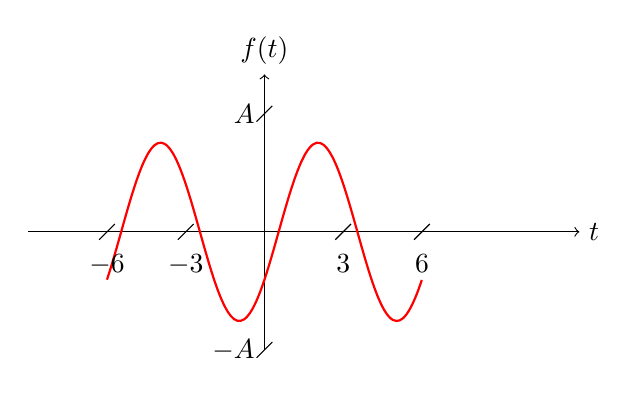
\begin{tikzpicture}
    %\draw (0,0) circle (1in);
    \draw[->] (-3.0,+0.0) -- (4.0,+0.0) node[right] {$t$};
    \draw[->] (+0.0,-1.5) -- (+0.0,+2.0) node[above] {$f(t)$};
    
    \draw[scale=1.0,domain=-2.0:2.0,samples=100,smooth,variable=\x,red,thick] plot ({\x},{-6/(3.141592*3.141592)*cos(\x*180.0*1)+3/(3.141592)*sin(\x*180.0*1)});
    
    \draw[-] (-2.0-0.1,-0.1)--(-2.0+0.1,0.1) node[midway, below, outer sep=5pt] {$-6$};
    \draw[-] (-1.0-0.1,-0.1)--(-1.0+0.1,0.1) node[midway, below, outer sep=5pt] {$-3$};
    \draw[-] (+1.0-0.1,-0.1)--(+1.0+0.1,0.1) node[midway, below, outer sep=5pt] {$3$};
    \draw[-] (+2.0-0.1,-0.1)--(+2.0+0.1,0.1) node[midway, below, outer sep=5pt] {$6$};
    \draw[-] (-0.1,+1.5-0.1)--(+0.1,+1.5+0.1) node[midway, left] {$A$};
    \draw[-] (-0.1,-1.5-0.1)--(+0.1,-1.5+0.1) node[midway, left] {$-A$};
    
    \end{tikzpicture}
\end{figure}

\TT{W przypadku sumowania do $k_{max}=3$ otrzymujemy}{A partial approximation of the $f(t)$ signal for $k_{max}=3$ results in:}

\begin{figure}[H]
    \centering
    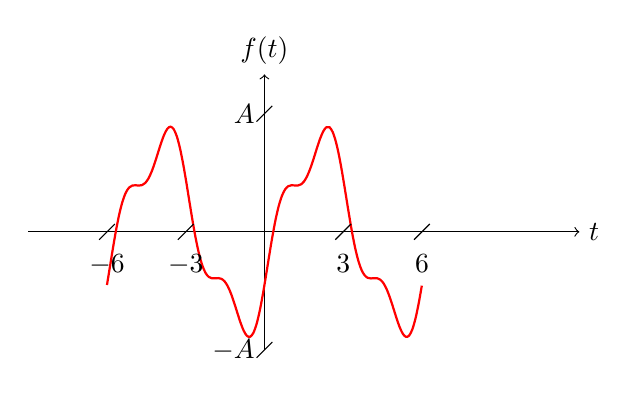
\begin{tikzpicture}
    %\draw (0,0) circle (1in);
    \draw[->] (-3.0,+0.0) -- (4.0,+0.0) node[right] {$t$};
    \draw[->] (+0.0,-1.5) -- (+0.0,+2.0) node[above] {$f(t)$};
    
    \draw[scale=1.0,domain=-2.0:2.0,samples=100,smooth,variable=\x,red,thick] plot ({\x},{-6/(3.141592*3.141592)*cos(\x*180.0*1)+3/(3.141592)*sin(\x*180.0*1) -6/(3.141592*3.141592*9)*cos(\x*180.0*3)+3/(3.141592*3)*sin(\x*180.0*3)});
    
    \draw[-] (-2.0-0.1,-0.1)--(-2.0+0.1,0.1) node[midway, below, outer sep=5pt] {$-6$};
    \draw[-] (-1.0-0.1,-0.1)--(-1.0+0.1,0.1) node[midway, below, outer sep=5pt] {$-3$};
    \draw[-] (+1.0-0.1,-0.1)--(+1.0+0.1,0.1) node[midway, below, outer sep=5pt] {$3$};
    \draw[-] (+2.0-0.1,-0.1)--(+2.0+0.1,0.1) node[midway, below, outer sep=5pt] {$6$};
    \draw[-] (-0.1,+1.5-0.1)--(+0.1,+1.5+0.1) node[midway, left] {$A$};
    \draw[-] (-0.1,-1.5-0.1)--(+0.1,-1.5+0.1) node[midway, left] {$-A$};
    
    \end{tikzpicture}
\end{figure}

\TT{W przypadku sumowania do $k_{max}=5$ otrzymujemy}{A partial approximation of the $f(t)$ signal for $k_{max}=5$ results in:}

\begin{figure}[H]
    \centering
    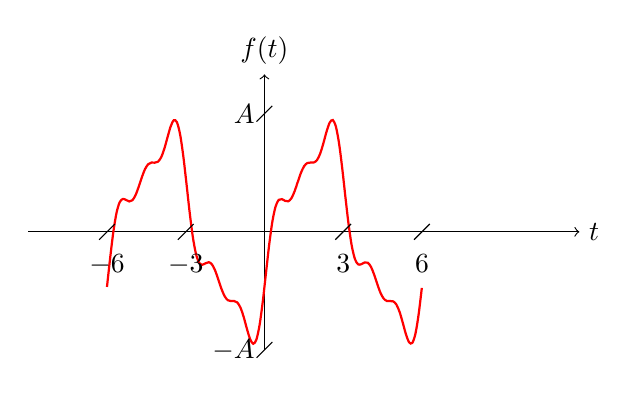
\begin{tikzpicture}
    %\draw (0,0) circle (1in);
    \draw[->] (-3.0,+0.0) -- (4.0,+0.0) node[right] {$t$};
    \draw[->] (+0.0,-1.5) -- (+0.0,+2.0) node[above] {$f(t)$};
    
    \draw[scale=1.0,domain=-2.0:2.0,samples=100,smooth,variable=\x,red,thick] plot ({\x},{-6/(3.141592*3.141592)*cos(\x*180.0*1)+3/(3.141592)*sin(\x*180.0*1) -6/(3.141592*3.141592*9)*cos(\x*180.0*3)+3/(3.141592*3)*sin(\x*180.0*3)
    -6/(3.141592*3.141592*25)*cos(\x*180.0*5)+3/(3.141592*5)*sin(\x*180.0*5)});
    
    \draw[-] (-2.0-0.1,-0.1)--(-2.0+0.1,0.1) node[midway, below, outer sep=5pt] {$-6$};
    \draw[-] (-1.0-0.1,-0.1)--(-1.0+0.1,0.1) node[midway, below, outer sep=5pt] {$-3$};
    \draw[-] (+1.0-0.1,-0.1)--(+1.0+0.1,0.1) node[midway, below, outer sep=5pt] {$3$};
    \draw[-] (+2.0-0.1,-0.1)--(+2.0+0.1,0.1) node[midway, below, outer sep=5pt] {$6$};
    \draw[-] (-0.1,+1.5-0.1)--(+0.1,+1.5+0.1) node[midway, left] {$A$};
    \draw[-] (-0.1,-1.5-0.1)--(+0.1,-1.5+0.1) node[midway, left] {$-A$};
    
    \end{tikzpicture}
\end{figure}

\TT{W przypadku sumowania do $k_{max}=7$ otrzymujemy}{A partial approximation of the $f(t)$ signal for $k_{max}=7$ results in:}

\begin{figure}[H]
    \centering
    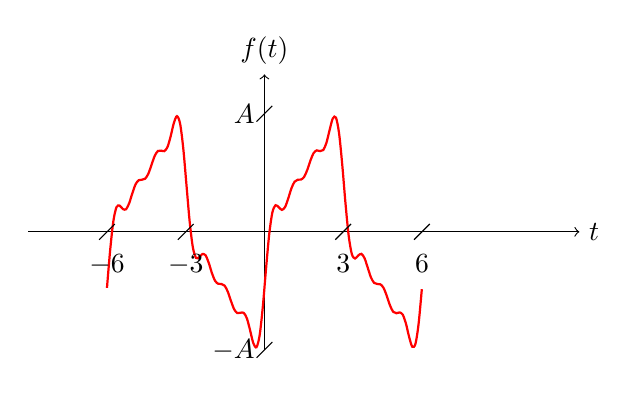
\begin{tikzpicture}
    %\draw (0,0) circle (1in);
    \draw[->] (-3.0,+0.0) -- (4.0,+0.0) node[right] {$t$};
    \draw[->] (+0.0,-1.5) -- (+0.0,+2.0) node[above] {$f(t)$};
    
    \draw[scale=1.0,domain=-2.0:2.0,samples=100,smooth,variable=\x,red,thick] plot ({\x},{-6/(3.141592*3.141592)*cos(\x*180.0*1)+3/(3.141592)*sin(\x*180.0*1) -6/(3.141592*3.141592*9)*cos(\x*180.0*3)+3/(3.141592*3)*sin(\x*180.0*3)
    -6/(3.141592*3.141592*25)*cos(\x*180.0*5)+3/(3.141592*5)*sin(\x*180.0*5)
    -6/(3.141592*3.141592*49)*cos(\x*180.0*7)+3/(3.141592*7)*sin(\x*180.0*7)});
    
    \draw[-] (-2.0-0.1,-0.1)--(-2.0+0.1,0.1) node[midway, below, outer sep=5pt] {$-6$};
    \draw[-] (-1.0-0.1,-0.1)--(-1.0+0.1,0.1) node[midway, below, outer sep=5pt] {$-3$};
    \draw[-] (+1.0-0.1,-0.1)--(+1.0+0.1,0.1) node[midway, below, outer sep=5pt] {$3$};
    \draw[-] (+2.0-0.1,-0.1)--(+2.0+0.1,0.1) node[midway, below, outer sep=5pt] {$6$};
    \draw[-] (-0.1,+1.5-0.1)--(+0.1,+1.5+0.1) node[midway, left] {$A$};
    \draw[-] (-0.1,-1.5-0.1)--(+0.1,-1.5+0.1) node[midway, left] {$-A$};
    
    \end{tikzpicture}
\end{figure}

\TT{W przypadku sumowania do $k_{max}=11$ otrzymujemy}{A partial approximation of the $f(t)$ signal for $k_{max}=11$ results in:}

\begin{figure}[H]
    \centering
    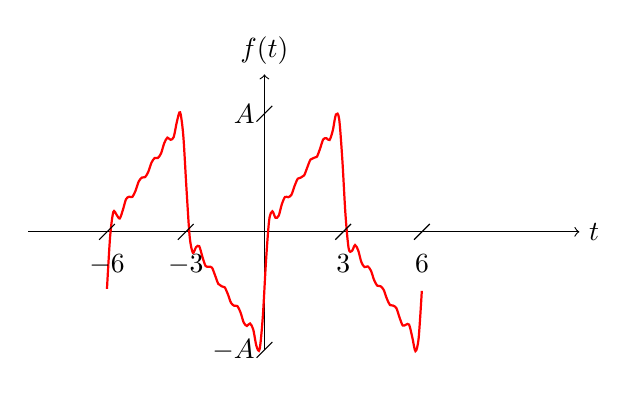
\begin{tikzpicture}
    %\draw (0,0) circle (1in);
    \draw[->] (-3.0,+0.0) -- (4.0,+0.0) node[right] {$t$};
    \draw[->] (+0.0,-1.5) -- (+0.0,+2.0) node[above] {$f(t)$};
    
    \draw[scale=1.0,domain=-2.0:2.0,samples=100,smooth,variable=\x,red,thick] plot ({\x},{-6/(3.141592*3.141592)*cos(\x*180.0*1)+3/(3.141592)*sin(\x*180.0*1) -6/(3.141592*3.141592*9)*cos(\x*180.0*3)+3/(3.141592*3)*sin(\x*180.0*3)
    -6/(3.141592*3.141592*25)*cos(\x*180.0*5)+3/(3.141592*5)*sin(\x*180.0*5)
    -6/(3.141592*3.141592*49)*cos(\x*180.0*7)+3/(3.141592*7)*sin(\x*180.0*7)
-6/(3.141592*3.141592*81)*cos(\x*180.0*9)+3/(3.141592*9)*sin(\x*180.0*9)
-6/(3.141592*3.141592*121)*cos(\x*180.0*11)+3/(3.141592*11)*sin(\x*180.0*11)});
    
    \draw[-] (-2.0-0.1,-0.1)--(-2.0+0.1,0.1) node[midway, below, outer sep=5pt] {$-6$};
    \draw[-] (-1.0-0.1,-0.1)--(-1.0+0.1,0.1) node[midway, below, outer sep=5pt] {$-3$};
    \draw[-] (+1.0-0.1,-0.1)--(+1.0+0.1,0.1) node[midway, below, outer sep=5pt] {$3$};
    \draw[-] (+2.0-0.1,-0.1)--(+2.0+0.1,0.1) node[midway, below, outer sep=5pt] {$6$};
    \draw[-] (-0.1,+1.5-0.1)--(+0.1,+1.5+0.1) node[midway, left] {$A$};
    \draw[-] (-0.1,-1.5-0.1)--(+0.1,-1.5+0.1) node[midway, left] {$-A$};
    
    \end{tikzpicture}
\end{figure}

\TT{W przypadku sumowania do $k_{max}=21$ otrzymujemy}{A partial approximation of the $f(t)$ signal for $k_{max}=21$ results in:}

\begin{figure}[H]
    \centering
    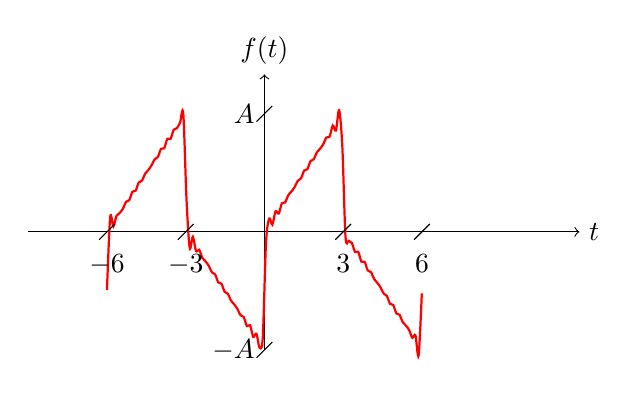
\begin{tikzpicture}
    %\draw (0,0) circle (1in);
    \draw[->] (-3.0,+0.0) -- (4.0,+0.0) node[right] {$t$};
    \draw[->] (+0.0,-1.5) -- (+0.0,+2.0) node[above] {$f(t)$};
    
    \draw[scale=1.0,domain=-2.0:2.0,samples=100,smooth,variable=\x,red,thick] plot ({\x},{-6/(3.141592*3.141592)*cos(\x*180.0*1)+3/(3.141592)*sin(\x*180.0*1) -6/(3.141592*3.141592*9)*cos(\x*180.0*3)+3/(3.141592*3)*sin(\x*180.0*3)
    -6/(3.141592*3.141592*25)*cos(\x*180.0*5)+3/(3.141592*5)*sin(\x*180.0*5)
    -6/(3.141592*3.141592*49)*cos(\x*180.0*7)+3/(3.141592*7)*sin(\x*180.0*7)
    -6/(3.141592*3.141592*81)*cos(\x*180.0*9)+3/(3.141592*9)*sin(\x*180.0*9)
    -6/(3.141592*3.141592*121)*cos(\x*180.0*11)+3/(3.141592*11)*sin(\x*180.0*11)
    -6/(3.141592*3.141592*169)*cos(\x*180.0*13)+3/(3.141592*13)*sin(\x*180.0*13)
    -6/(3.141592*3.141592*225)*cos(\x*180.0*15)+3/(3.141592*15)*sin(\x*180.0*15)
    -6/(3.141592*3.141592*289)*cos(\x*180.0*17)+3/(3.141592*17)*sin(\x*180.0*17)
    -6/(3.141592*3.141592*361)*cos(\x*180.0*19)+3/(3.141592*19)*sin(\x*180.0*19)
    -6/(3.141592*3.141592*441)*cos(\x*180.0*21)+3/(3.141592*21)*sin(\x*180.0*21)});
    
    \draw[-] (-2.0-0.1,-0.1)--(-2.0+0.1,0.1) node[midway, below, outer sep=5pt] {$-6$};
    \draw[-] (-1.0-0.1,-0.1)--(-1.0+0.1,0.1) node[midway, below, outer sep=5pt] {$-3$};
    \draw[-] (+1.0-0.1,-0.1)--(+1.0+0.1,0.1) node[midway, below, outer sep=5pt] {$3$};
    \draw[-] (+2.0-0.1,-0.1)--(+2.0+0.1,0.1) node[midway, below, outer sep=5pt] {$6$};
    \draw[-] (-0.1,+1.5-0.1)--(+0.1,+1.5+0.1) node[midway, left] {$A$};
    \draw[-] (-0.1,-1.5-0.1)--(+0.1,-1.5+0.1) node[midway, left] {$-A$};
    
    \end{tikzpicture}
\end{figure}

\TT{W granicy sumowania do $k_{max}=\infty$ otrzymujemy oryginalny sygnał.}{Approximation of the $f(t)$ signal for $k_{max}=\infty$ results in oryginal signal.}

\end{task}